\subsection*{Model}
The function described in this problem is the following
\begin{equation*}
    \begin{aligned}
    & F(\mathbf{x}) = \frac{1}{2} \sum_{k=1}^{n} f_k^2(x) \\
    & f_k(\mathbf{x}) = 10 \left(x_k^2 - x_{k+1}\right), \quad  & \mod (k,2) = 1\\   
    & f_n(\mathbf{x}) = x_{k_1} -1, \quad & \mod(k,2) = 0
    \end{aligned}
\end{equation*}
where $n$ denotes the dimensionality of the input vector $\mathbf{x}$. As convention, we set $x_{n+1} = x_1$ when it is necessary, that is when the dimensionality $n$ is an odd number.
\\ The starting point for the minimization is the vector $\mathbf{x}_0 = [-1.2, 1, -1.2, 1, \ldots]$.

In order to compute the derivatives of this problem we have to consider separately the cases when $n$ is even or odd. In the first case, the gradient of the function is given by
\begin{align*}
    &\frac{\partial F}{\partial x_k} (\mathbf{x}) = \frac{\partial}{\partial x_k} \left[\frac{1}{2} f_{k-1}^2(\mathbf{x})\right] = - 100 (x_{k-1}^2 - x_k) \quad & \mod(k,2) = 0 \\
    & \frac{\partial F}{\partial x_k} (\mathbf{x}) = \frac{\partial}{\partial x_k} \left[\frac{1}{2} f_{k}^2(\mathbf{x}) + \frac{1}{2} f_{k+1}^2(\mathbf{x})\right] = 200x_k (x_k^2 - x_{k+1}) + (x_k -1)\quad & \mod(k,2) = 1
\end{align*}

If the dimensionality $n$ is odd, the only changement is in the first component of the gradient, which becomes
$$ \frac{\partial F}{\partial x_1} (\mathbf{x})  = \frac{\partial}{\partial x_k} \left[\frac{1}{2} f_{k}^2(\mathbf{x}) + \frac{1}{2} f_{k+1}^2(\mathbf{x}) + \frac{1}{2}f_n^2(\mathbf{x}) \right] = 200x_1 (x_1^2 - x_{2}) + (x_1 -1)  - 100(x_n^2 - x_1)$$

Looking at the structure of the problem we are considering, it is obvious that the Hessian matrix is a sparse matrix whose particular structure depends again on wheter $n$ is even or odd. In the first case, the Hessian is a block tridiagonal matrix with the following non-zero terms
\begin{align*}
    \frac{\partial^2 F}{\partial x_k^2} (\mathbf{x}) &= 100, & \frac{\partial^2 F}{\partial x_k \partial x_{k+1}} (\mathbf{x}) &= 0, & \frac{\partial^2 F}{\partial x_k \partial x_{k-1}} (\mathbf{x}) &= -200x_{k-1} & \mod(k,2) &= 0 \\
    \frac{\partial^2 F}{\partial x_k^2} (\mathbf{x}) &= 600x_k^2 - 200x_{k+1} + 1, & \frac{\partial^2 F}{\partial x_k \partial x_{k+1}} (\mathbf{x}) &= -200x_k, & \frac{\partial^2 F}{\partial x_k \partial x_{k-1}} (\mathbf{x}) &= 0 & \mod(k,2) &= 1 \\
\end{align*}

If $n$ is odd, there are two changements in the Hessian matrix: the derivative $\frac{\partial^2 F}{\partial x_1^2} (\mathbf{x}) $ is affected by the presence of $x_1$ in the term $f_n()$ and the extremal diagonals are not zero anymore. We report the terms of the Hessian matrix that differs from the previous case
\begin{align*}
    \frac{\partial^2 F}{\partial x_1^2}  (\mathbf{x}) &= 600x_k^2 - 200x_{k+1} + 101 \\
    \frac{\partial^2 F}{\partial x_n \partial x_1} (\mathbf{x}) &= \frac{\partial^2 F}{\partial x_1 \partial x_n} (\mathbf{x}) = -200x_n
\end{align*}


By analyzing the derivatives of the problem, we can deduce that the gradient of the function is nullified by the vector composed of ones which also nullifies the value of $F(\mathbf{x})$. 


 
\medskip
\subsection*{Nealder Mead Method}
We now report a table showing some general results obtained by running the Nealder Mead method on the problem.
\begin{figure*}[htbp]
    \centering
    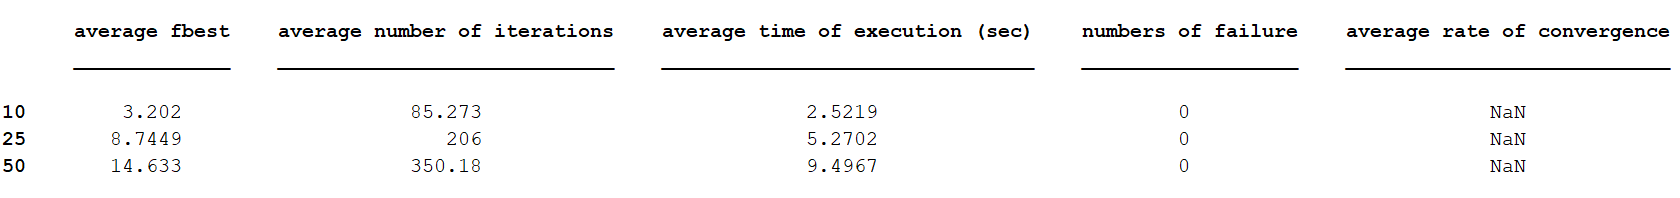
\includegraphics[width = 0.9\textwidth]{img/pb25_SX_table.png}
    \caption{Resultats obtained by running the symplex method on the problem $25$.}
\end{figure*}

















\medskip
\subsection*{Modified Newton Method - Exact Derivatives}
\begin{figure*}[htbp]
    \centering
    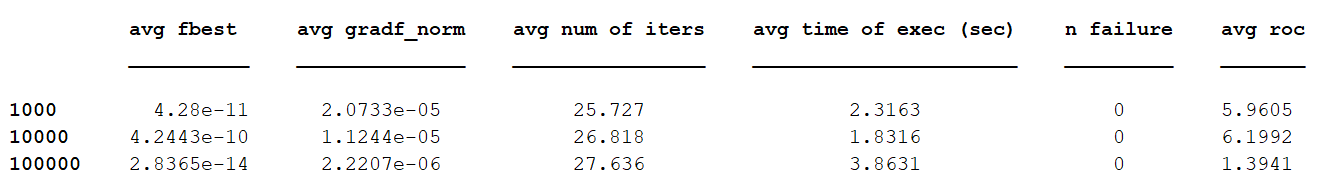
\includegraphics[width = 0.9\textwidth]{img/pb25_MN_table.png}
    \caption{Resultats obtained by running the Modified Newton method on the problem $25$ using the exact derivatives.}
\end{figure*}



\medskip
\subsection*{Modified Newton Method - Approximated Derivatives}